
\section{Introduction}\label{subsub:Intro-Main}

\citet{Ronquist2012a} 

Exercise is in Section \ref{sect:RB-ExerciseMain}.

\subsection{Models}\label{subsect:Intro-Models}

The focus of this tutorial is to introduce you to specifying the models used in an analysis of fossil and extant taxa. 
\citet{Hoehna2014b}

\begin{figure}[h!]
\centering
\fbox{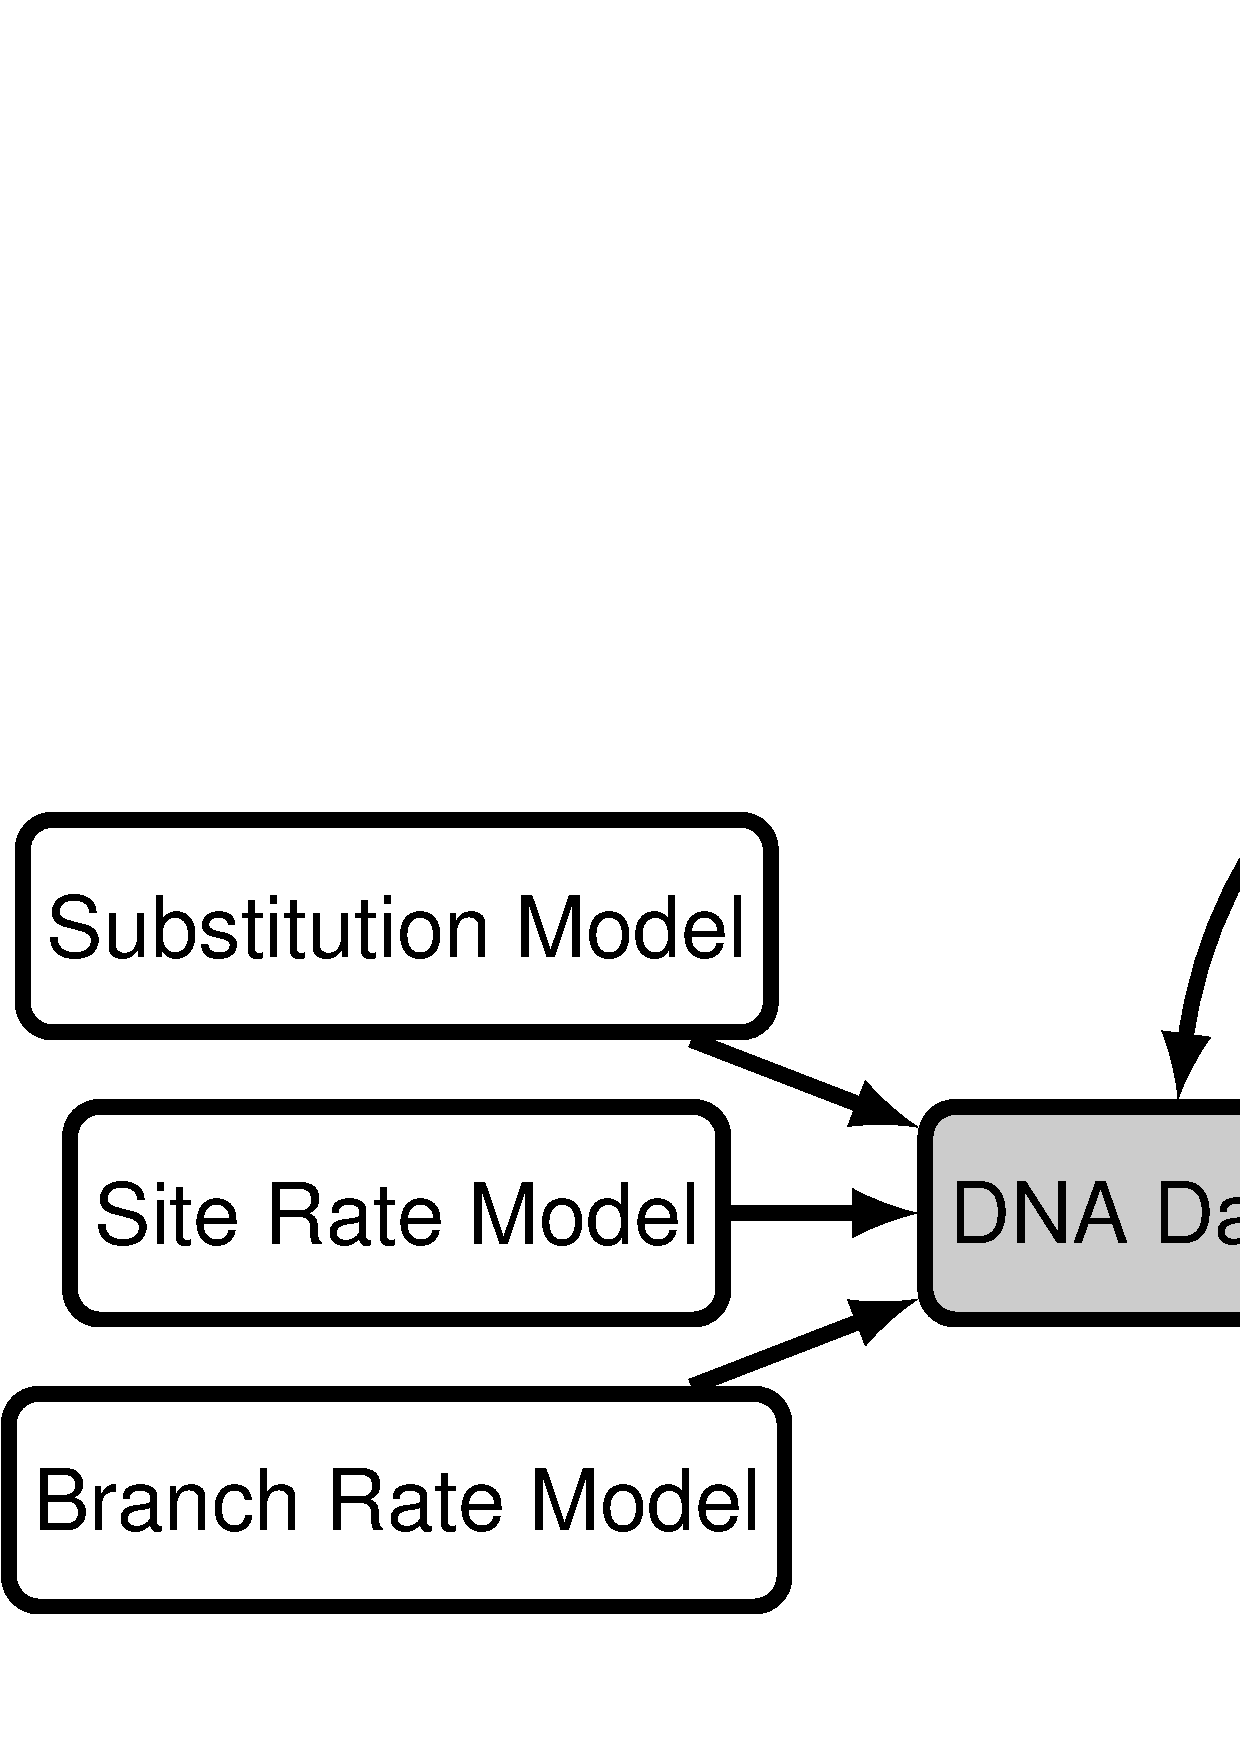
\includegraphics[width=\textwidth,angle=0]{\ResourcePath figures/tikz/full_model_modular}}
\caption{\small  }
\label{fig:fbd_gm}
\end{figure}


\subsubsection{Lineage Diversification and Sampling}\label{subsub:Intro-FBD}

Birth-death processes and FBD

\begin{figure}[h!]
\centering
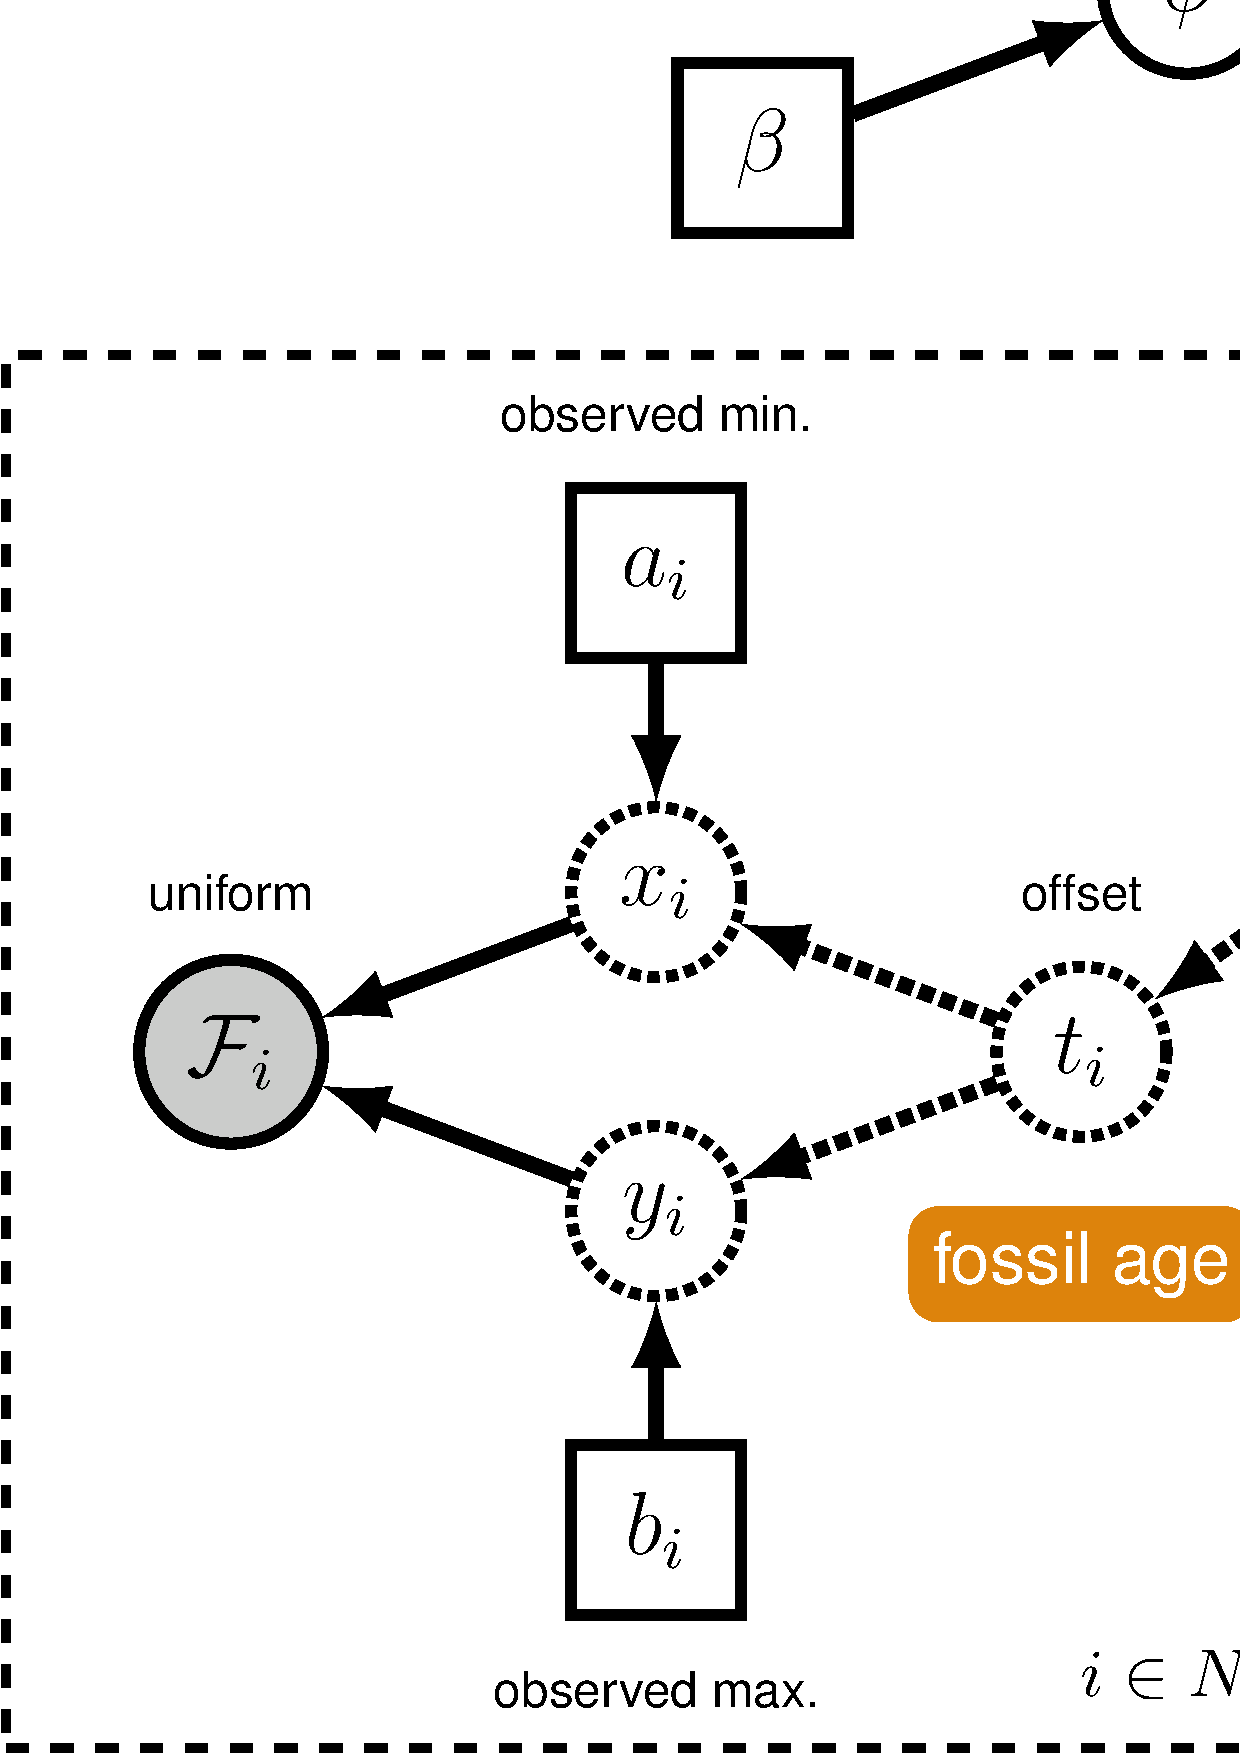
\includegraphics[scale=0.3,angle=0]{\ResourcePath figures/tikz/fbd_gm}
\caption{\small A graphical model of the fossilized birth death process. In this model, the speciation, extinction and fossilization rates are drawn from exponential distributions, while the origin time and fossil ages are uniformly distributed. }
\label{fig:fbd_gm}
\end{figure}


\subsubsection{Sequence Evolution}\label{subsub:Intro-GTR}

In this tutorial, we will analyze our molecular data using a general time-reversible model of nucleotide evolution and gamma-distributed rate heterogeneity across sites.
This model of sequence evolution is covered thoroughly in the \href{https://github.com/revbayes/revbayes_tutorial/raw/master/tutorial_TeX/RB_CTMC_Tutorial/RB_CTMC_Tutorial.pdf}{RB\_CTMC\_Tutorial}.

\subsubsection{Morphological Character Change}\label{subsub:Intro-Morpho}

The incorporation of morphological data from fossils into phylogenetic analyses allows us to directly observe organisms that existed in the past.
The Mk model \citep{Lewis2001} uses a generalized Jukes-Cantor matrix to allow for the incorporation of morphology into likelihood and Bayesian analyses.
One key assumption of this model is that characters exhibit symmetrical change - that a given character is as likely to transition from a one state to another as it is to reverse.
For example, this assumption applied to a binary character would mean that a change from a 0 state to a 1 state is as likely as a change from a 1 state to a 0 state. \par
In the tutorial, we will relax this assumption through the use of a prior on stationary state frequencies. 
This prior is visualized in Fig. \ref{fig:morpho_gm}. 
\begin{figure}[h!]
\centering
\fbox{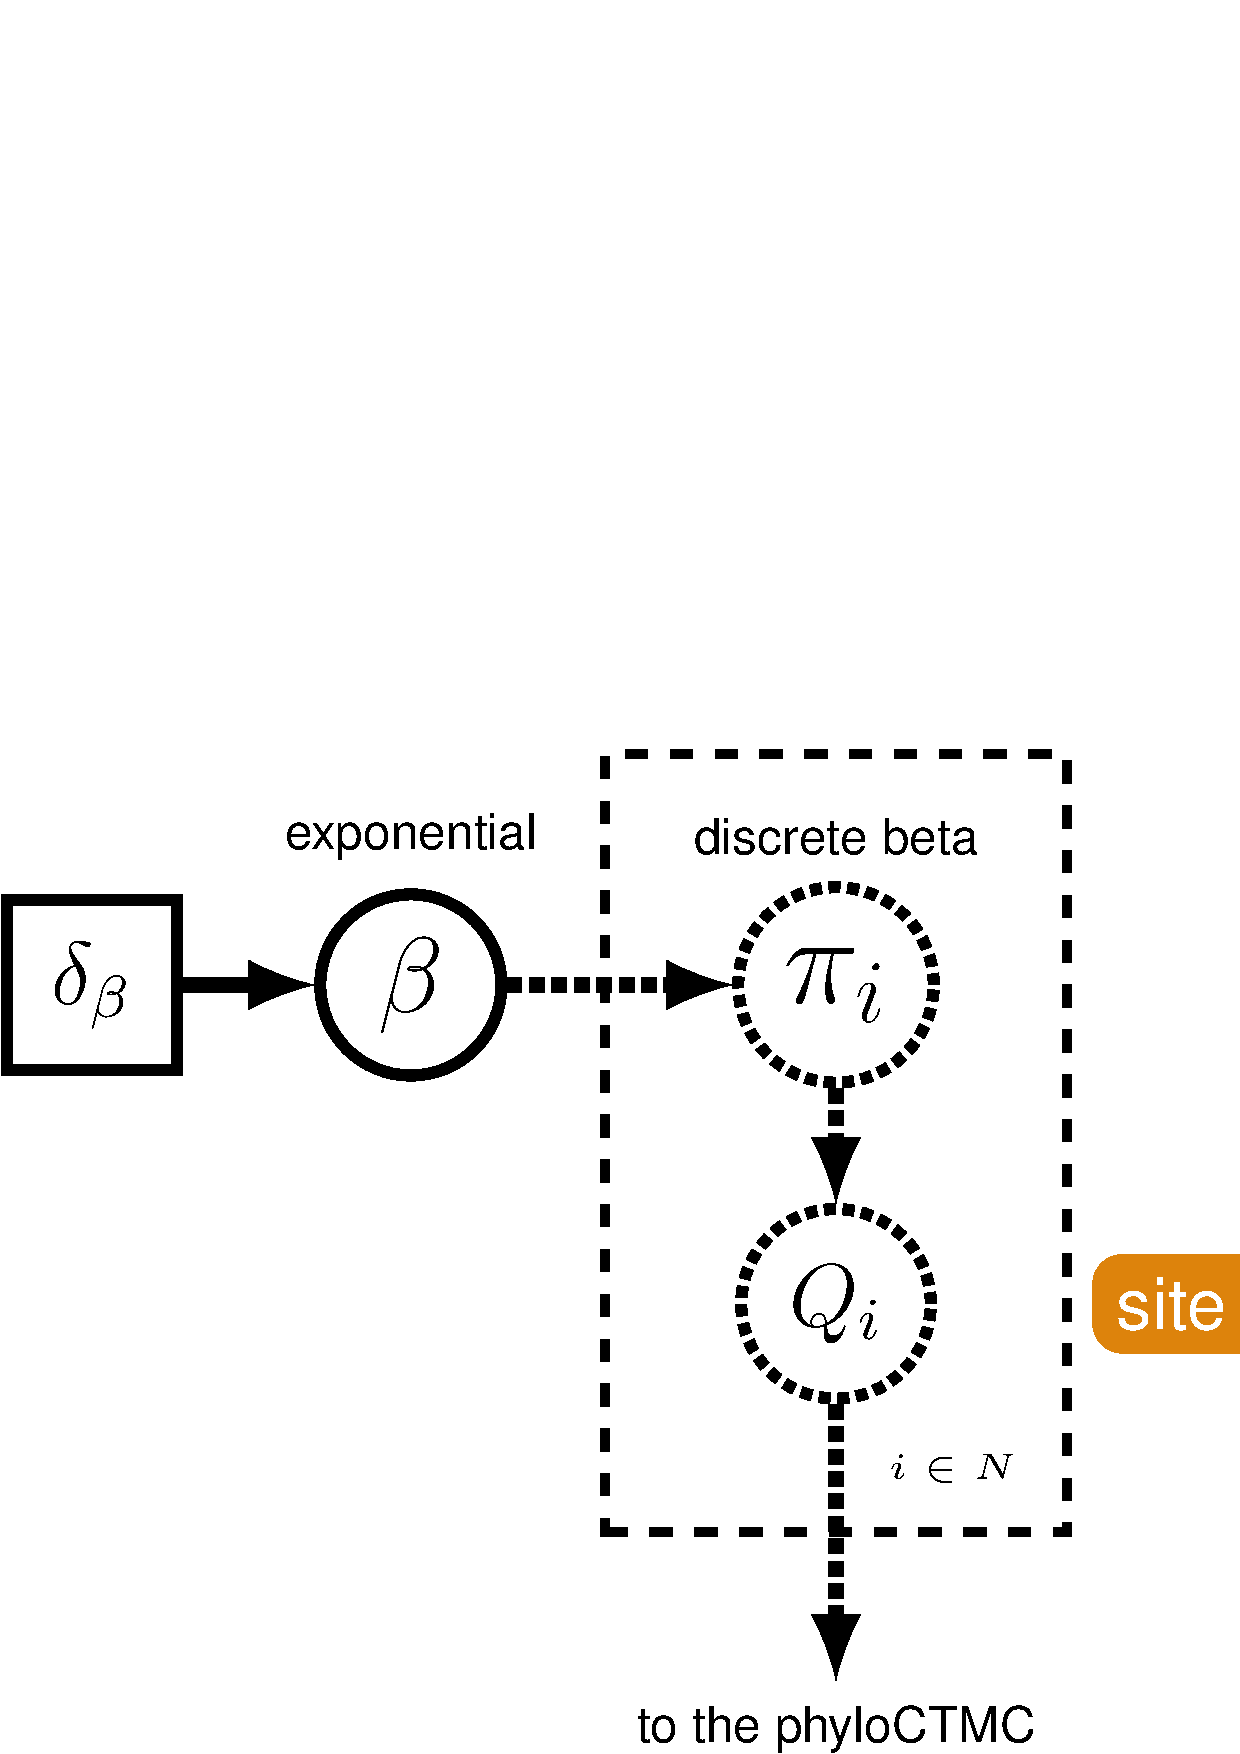
\includegraphics[scale=0.3,angle=0]{\ResourcePath figures/tikz/morpho_gm}}
\caption{\small A graphical model of the Beta-distributed frequencies across sites model. In this model, stationary state frequencies are drawn from a discrete Beta distribution and used to generate Q-matrices that allow character change asymmetry.}
\label{fig:morpho_gm}
\end{figure}
All of the morphological data we are working with in this tutorial are binary.  
Therefore, we can draw the stationary state frequencies of our 0 and 1 characters from a Beta distribution. 
Using the stationary state frequencies drawn from the Beta distribution, we can then create new Q-matrices that allow for asymmetrical change in characters states (i.e., for changing from state 0 to state 1 to be more likely than changing from state 1 to state 0, or vice versa). 
We can do multiple draws from the Beta distribution, creating multiple different Q-matrices per datset.
This allows for heterogeneity in character change asymmetry across the dataset. 
Likewise, we will use the Gamma distributed rate heterogeneity (described in \href{https://github.com/revbayes/revbayes_tutorial/raw/master/tutorial_TeX/RB_CTMC_Tutorial/RB_CTMC_Tutorial.pdf}{RB\_CTMC\_Tutorial}) to allow for different characters to evolve at different rates.\par

Because of the way morphological data are collected, we need to exercise caution in how we model the data. 
Traditionally, phylogenetic trees were built from morphological data using parsimony. 
Therefore, characters were collected to be parsimony informative - that is, to be useful for discriminating between phylogenetic hypotheses under the maximum parsimony criterion.
This means that many morphological datasets do not contain invariant characters or autapomorphies, as these cannot be used to discriminate among hypotheses under parsimony. 
By excluding these low rate of evolution characters, the estimated branch lengths can be inflated \citep{Felsenstein1992,Lewis2001}.
Therefore, it is important to use models that can condition on the coding bias. 
RevBayes has two ways of doing this: one is used for datasets in which only parsimony informative characters are observed; the other is for datasets in which parsimony informative characters and non-parsimony informative variable characters (such as autapomorphies) are observed. \par


\subsubsection{Lineage-Specific Rates of Evolution}\label{subsub:Intro-UExp}

Rates of nucleotide sequence evolution can vary widely among lineages, and so models that account for this variation by relaxing the assumption of a strict molecular clock can allow for more accurate estimates of substitution rates and divergence times \citep{Drummond2006}.
The simplest type of relaxed clock model assumes that lineage-specific substitution rates are independent or ``uncorrelated''.
One example of such an uncorrelated relaxed model is the ``Uncorrelated exponential relaxed clock'' (or UExp), in which the substitution rate for each lineage is assumed to be independent and identically distributed according to an exponential density (depicted in Fig. \ref{fig:uexp_gm}).
This is the model that we will use in this tutorial.
Another possible uncorrelated relaxed clock model is the uncorrelated lognormal model, described in the \href{https://github.com/revbayes/revbayes_tutorial/raw/master/tutorial_TeX/RB_Dating_Tutorial/RB_Dating_Tutorial.pdf}{RB\_Dating\_Tutorial}.
\begin{figure}[h!]
\centering
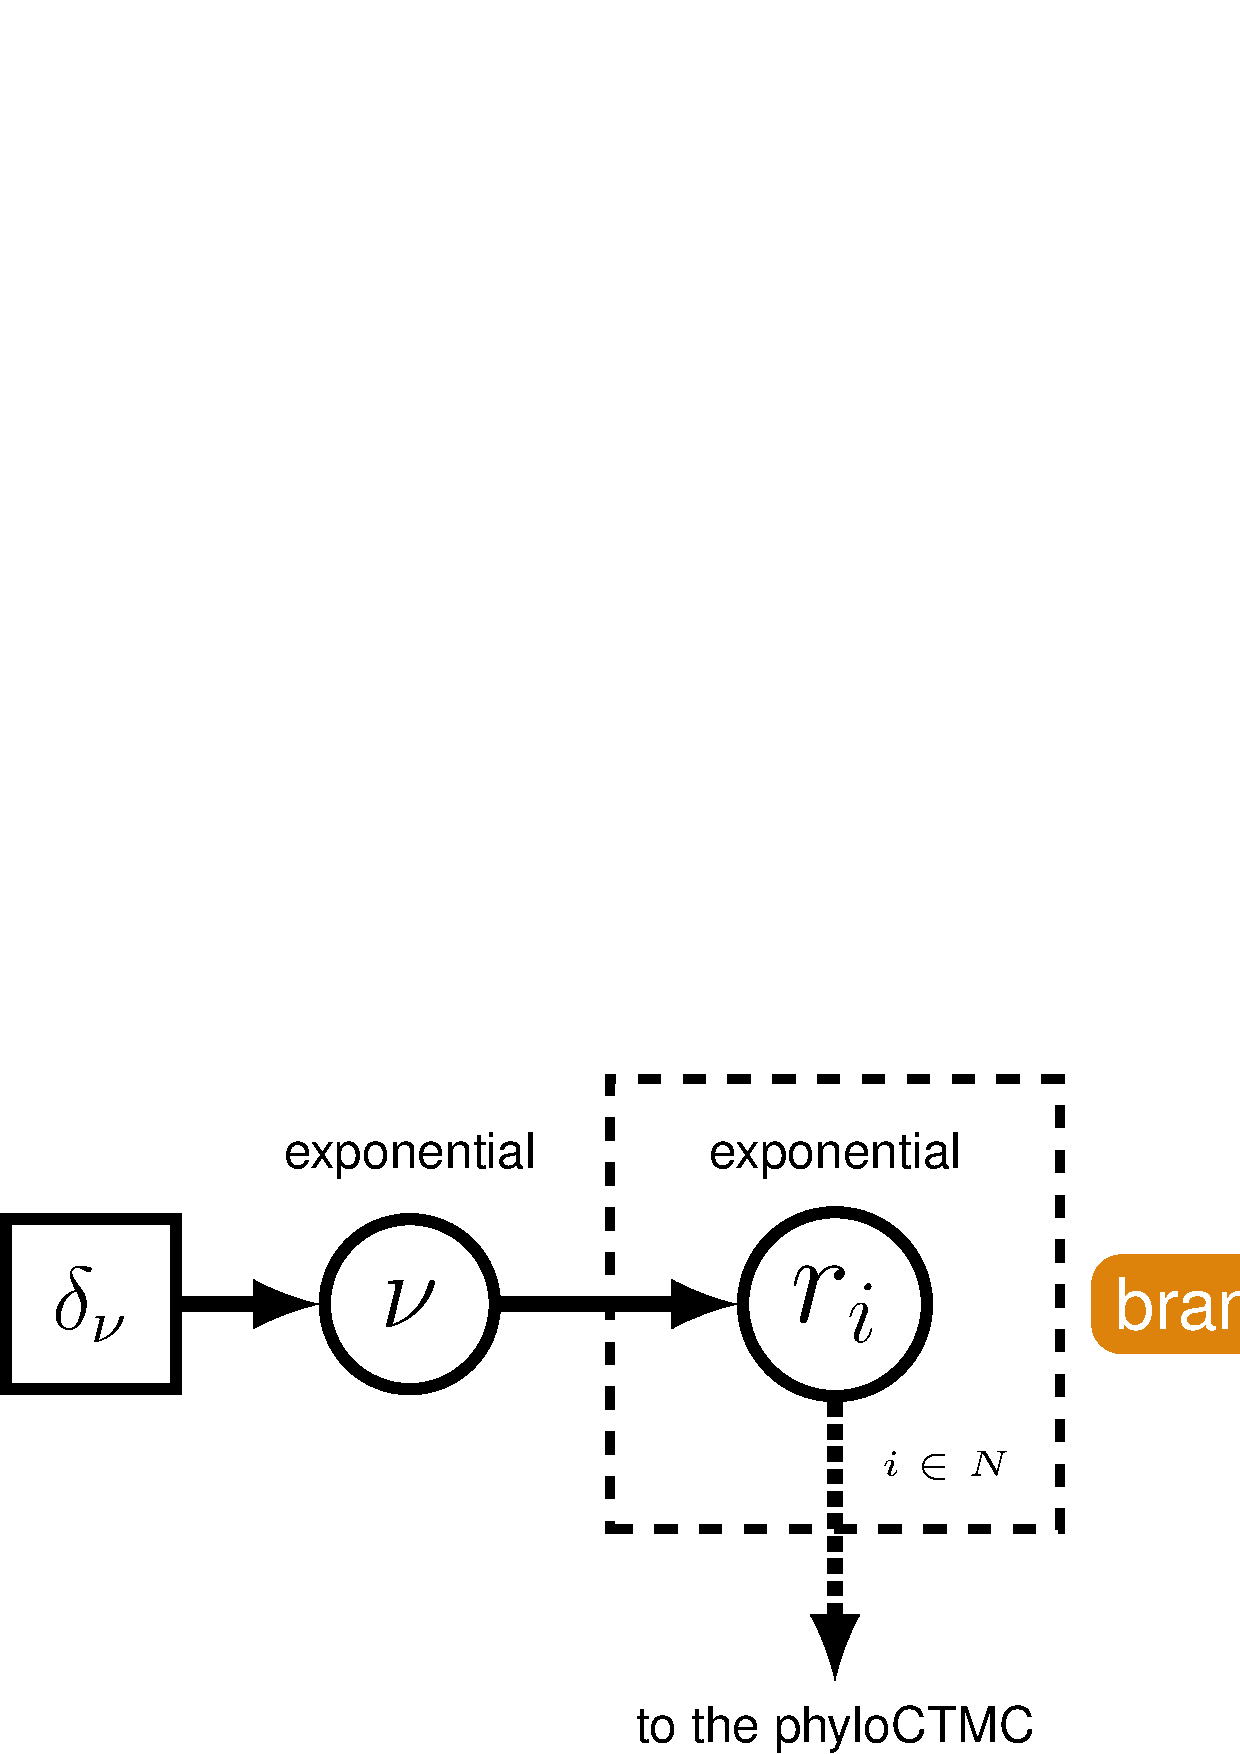
\includegraphics[scale=0.3,angle=0]{\ResourcePath figures/tikz/uexp_gm}
\caption{\small A graphical model of the uncorrelated exponential relaxed clock model. In this model, the clock rate on each branch is independent and identically distributed according to an exponential density with mean drawn from an exponential hyperprior distribution. }
\label{fig:uexp_gm}
\end{figure}


\section{Prerequisites}

What do you need to know before doing this?

\subsection{Requirements}
We assume that you have read and hopefully completed the following tutorials:
\begin{itemize}
\item \href{https://github.com/revbayes/revbayes_tutorial/raw/master/tutorial_TeX/RB_Getting_Started/RB_Getting_Started.pdf}{RB\_Getting\_Started}
\item \href{https://github.com/revbayes/revbayes_tutorial/raw/master/tutorial_TeX/RB_Basics_Tutorial/RB_Basics_Tutorial.pdf}{RB\_Basics\_Tutorial}
\end{itemize}
Note that the RB\_Basics\_Tutorial introduces the basic syntax of \Rev but does not cover any phylogenetic models.
You may skip the RB\_Basics\_Tutorial if you have some familiarity with \R.
We tried to keep this tutorial very basic and introduce all the language concepts on the way.
You may only need the RB\_Basics\_Tutorial for a more in-depth discussion of concepts in \Rev.




\section{Exercise: Estimating the Phylogeny and Divergence Times of Fossil and Extant Bears}\label{sect:RB-ExerciseMain}

In this exercise, we will combine different types of data from 22 species of bears to estimate a posterior distribution of calibrated time trees.
The dataset we will use encompasses 8 extant species and 14 fossil species, consisting of morphological data for 18 species, nucleotide sequence data from 10 species, and stratigraphic fossil range data for all 14 fossil species.
Two fossil species do not have any morphological or molecular data.

\subsection{Data files}\label{subsect:RB-DataFiles}

We provide the data files which we will use in this tutorial.
You may want to use your own data instead.
In the \cl{data} folder, you will find the following files
\begin{itemize}[noitemsep,topsep=0pt]
\item \cl{bears\_taxa.tsv}: a tab-separated table listing every bear species (both fossil and extant) and their occurrence dates. For extant taxa, the occurrence date is \cl{0.0} (\IE the present) and for fossil species, the occurrence date is equal to the mean of the age range (the ranges are defined in a separate file).
\item \cl{bears\_cytb.nex}: an alignment in NEXUS format of 1,000 bp of cytochrome b sequences for 10 bear species. This alignment includes 8 living bears and 2 extinct sub-fossil bears.
\item \cl{bears\_morphology.nex}: a matrix of 62 discrete, binary (coded \cl{0} or \cl{1}) morphological characters for 18 species of fossil and extant bears.
\item \cl{bears\_fossil\_intervals.tsv}: a tab-separated table containing the age ranges (minimum and maximum in millions of years) for 14 fossil bears.
\end{itemize}


\bigskip
\subsection{Getting Started}\label{subsect:RB-GetStart}

{\begin{framed}
On your own computer, create a directory called {\textcolor{red}{\cl{RB\_TotalEvidenceDating\_FBD\_Tutorial}}} (or any name you like). 

In this directory download and unzip the archive containing the data files: \href{www.revbayes.com}{\cl{data.zip}}.

Additionally, create a new directory (in \cl{RB\_TotalEvidenceDating\_FBD\_Tutorial}) called {\textcolor{red}{\cl{scripts}}}
\end{framed}}

When you execute \RevBayes in this exercise, you will do so within the main directory you created (\cl{RB\_TotalEvidenceDating\_FBD\_Tutorial}).

%TODO Stuff about how to start or Rev basics?

%We will complete this analysis in \RevBayes by entering the \Rev code interactively. 
%
%Note that some PDF viewers render some characters differently and if you copy/paste directly from this document, you may introduce erroneous characters. 
%This can cause commands to fail. 
%For learning, it's often better to `live code' and type the commands in manually, rather than copying and pasting. 
%
%Hints for navigating in the \RevBayes console:
%\begin{itemize}[noitemsep,topsep=0pt]
%    \item \cl{Ctrl+A} -- jump to the beginning of the line
%    \item \cl{Ctrl+E} -- jump to the end of the line
%    \item Pressing the up key will pull up previous commands, and allow you to edit them
%    \item If you enter the first few letters of a \RevBayes keyword and then the \textsc{Tab} key, this will `autocomplete' the remaining letters.
%    \item Help -- if you type \cl{?} followed immediately by a \RevBayes keyword, this will print the help pages for that keyword to the screen. (Example \cl{?dnBDP})
%\end{itemize}
%%In \RevBayes, \cl{Ctrl+A} allows you to jump to the start of the command, if you need to delete extra characters from the front of a line. \cl{Ctrl+E} allows you to jump to the end of a command. Pressing the up key will pull up previous commands, and allow you to edit them. If you do choose to copy and paste in commands, doing that from the tutorial script file will cause fewer errors. 

\bigskip

\subsection{Creating \Rev Files}\label{subsect:RB-CreatingFiles}

For complex models and analyses, it is best to create \Rev script files that will contain all of the model parameters, moves, and functions. 
In this exercise, you will work primarily in your text editor and create a set of modular files that will be easily managed and interchanged.
You will write the following files from scratch in a text editor\footnote{If you do not already have a good text editor that you like, we recommend one that has features for syntax coloring, easy navigation between different files, line numbers, etc.
A good option is \href{http://www.sublimetext.com/}{Sublime Text}, which is available for Mac OSX, Windows, and Linux.} and save them in the \cl{scripts} directory:
\begin{itemize}[noitemsep,topsep=0pt]
\item \cl{mcmc\_TEFBD.Rev}: the master \Rev file that loads the data, the separate model files, and specifies the monitors and MCMC sampler.
\item \cl{model\_FBDP\_TEFBD.Rev}: specifies the model parameters and moves required for the fossilized birth-death prior on the tree topology, divergence times, fossil occurrence times, and diversification dynamics.
\item \cl{model\_UExp\_TEFBD.Rev}: specifies the components of the uncorrelated exponential model of lineage-specific substitution rate variation.
\item \cl{model\_GTRG\_TEFBD.Rev}: specifies the parameters and moves for the general time-reversible model of sequence evolution with gamma-distributed rates across sites (GTR+$\Gamma$).
\item \cl{model\_Morph\_TEFBD.Rev}: specifies the model describing discrete morphological character change (binary characters) under a strict morphological clock. 
\end{itemize}

All of the files that you will create are also provided in the \RevBayes tutorial repository\footnote{\url{https://github.com/revbayes/revbayes_tutorial/tree/master/RB_TotalEvidenceDating_FBD_Tutorial/scripts}}. 
Please refer to these files to verify or troubleshoot your own scripts. 
%TODO add link to scripts


\bigskip
\subsection{Start the Master \Rev File and Import Data}\label{subsect:RB-StartMasterRev}



{\begin{framed}
Open your text editor and create the master \Rev file called {\textcolor{red}{\cl{mcmc\_TEFBD.Rev}}} in the \cl{scripts} directory.

Enter the \Rev code provided in this section in the new model file.
\end{framed}}

The file you will begin in this section will be the one you load into \RevBayes when you've completed all of the components of the analysis.
In this section you will begin the file and write the \Rev commands for loading in the taxon list and managing the data matrices.
Then, starting in Section \ref{subsect:RB-ModelFBD}, you will move on to writing module files for each of the model components. 
Once the model files are complete, you will return to editing \cl{mcmc\_TEFBD.Rev} and complete the \Rev script with the instructions given in Section \ref{subsect:RB-CompleteMCMC}.

%{\footnotesize{This file is provided in the \RevBayes tutorial repository: \href{https://github.com/revbayes/revbayes_tutorial/blob/master/RB_TotalEvidenceDating_FBD_Tutorial/scripts/mcmc_TEFBD.Rev}{\cl{mcmc\_TEFBD.Rev}}.}}

\medskip
\subsubsection{Load Taxon List}\label{subsub:RB-TaxList}

Begin the \Rev script by loading in the list of taxon names from the \cl{bears\_taxa.tsv} file using the \cl{readTaxonData()} function.
\begin{snugshade*}
\begin{lstlisting}
taxa <- readTaxonData("data/bears_taxa.tsv")
\end{lstlisting}
\end{snugshade*}
This function reads a tab-delimited file and creates a variable called \cl{taxa} that is a list of all of the taxon names relevant to this analysis. 
This list includes all of the fossil and extant bears.



\medskip
\subsubsection{Load Data Matrices}\label{subsub:RB-LoadData}

\RevBayes uses the function \cl{readDiscreteCharacterData()} to load a data matrix to the workspace from a formatted file. 
This function can be used for both molecular sequences and discrete morphological characters.

Load the cytochrome-b sequences from file and assign the data matrix to a variable called \cl{cytb}.
{\tt \begin{snugshade*}
\begin{lstlisting}
cytb <- readDiscreteCharacterData("data/bears_cytb.nex") 
\end{lstlisting}
\end{snugshade*}}

Next, import the morphological character matrix and assign it to the variable \cl{morpho}. 
{\tt \begin{snugshade*}
\begin{lstlisting}
morpho <- readDiscreteCharacterData("data/bears_morphology.nex")
\end{lstlisting}
\end{snugshade*}}

 

\medskip
\subsubsection{Add Missing Taxa}\label{subsub:RB-AddMissing}

In the descriptions of the files in Section \ref{subsect:RB-DataFiles}, we mentioned that the two data matrices have different numbers of taxa. 
Thus, we must add any taxa that are not found in the molecular (\cl{cytb}) partition (\IE are only found in the fossil data) to that data matrix as missing data, and do the same with the morphological data partition (\cl{morpho}).
In order for all the taxa to appear on the same tree, they all need to be part of the same dataset, as opposed to present in separate datasets. 
This ensures that there is a unified taxon set that contains all of our tips.
{\tt \begin{snugshade*}
\begin{lstlisting}
cytb.addMissingTaxa( taxa )
morpho.addMissingTaxa( taxa )
\end{lstlisting}
\end{snugshade*}}


\medskip
\subsubsection{Create Helper Variables}\label{subsub:RB-mviVar}

Before we begin writing the \Rev scripts for each of the model components, we need to instantiate a couple ``helper variables'' that will be used by downstream parts of our model specification files. 
These variables will be used in more than one of the module files so it's best to initialize them in the master file.

Create a new constant node called \cl{n\_taxa} that is equal to the number of species in our analysis (22). 
{\tt \begin{snugshade*}
\begin{lstlisting}
n_taxa <- taxa.size() 
\end{lstlisting}
\end{snugshade*}}

Next, create a \textit{workspace variable} called \cl{mvi}. 
This variable is an iterator that will build a vector containing all of the MCMC moves used to propose new states for every stochastic node in the model graph. 
Each time a new move is added to the vector, \cl{mvi} will be incremented by a value of \cl{1}.
{\tt \begin{snugshade*}
\begin{lstlisting}
mvi = 1
\end{lstlisting}
\end{snugshade*}}
One important distinction here is that \cl{mvi} is part of the \RevBayes workspace and not the hierarchical model. 
Thus, we use the workspace assignment operator \cl{=} instead of the constant node assignment \cl{<-}. 

{\begin{framed}
Save your current working version of \cl{mcmc\_TEFBD.Rev} in the \cl{scripts} directory.

We will now move on to the next \Rev file and will complete \cl{mcmc\_TEFBD.Rev} in Section \ref{subsect:RB-CompleteMCMC}.
\end{framed}}


\bigskip
\subsection{The Fossilized Birth-Death Process}\label{subsect:RB-ModelFBD}

{\begin{framed}
Open your text editor and create the fossilized birth-death model file called {\textcolor{red}{\cl{model\_FBDP\_TEFBD.Rev}}} in the \cl{scripts} directory.

Enter the \Rev code provided in this section in the new model file.
\end{framed}}

\subsubsection{Speciation and Extinction Rates}\label{subsub:RB-FBD-SpeciationExtinction}

Two key parameters of the FBD process are the speciation rate (the rate at which lineages are added to the tree) and the extinction rate (the rate at which lineages are removed from the tree). 
We'll place exponential priors on both of these values. 
%An exponential prior with a $\lambda$ =  10 places a higher probability on values closer to zero than one for these parameters. 
Each parameter is assumed to be drawn independently from a different exponential distribution with rates $\delta_{\lambda}$ and $\delta_{\mu}$ respectively (see Fig.\ \ref{fig:fbd_gm}). 
Here, we will assume that $\delta_{\lambda} = \delta_{\mu} = 10$. 
Note that an exponential distribution with $\delta = 10$ has an expected value (mean) of $1/10$. 
{\tt \begin{snugshade*}
\begin{lstlisting}
speciation_rate ~ dnExponential(10)
extinction_rate ~ dnExponential(10)
\end{lstlisting}
\end{snugshade*}}

For every stochastic node we declare, we must also specify proposal algorithms (called \textit{moves}) to sample the value of the parameter in proportion to its posterior probability.
If a move is not specified for a stochastic node, then it will not be estimated, but fixed to its initial value. 

The rate parameters for extinction and speciation are both real, positive numbers (\IE floating point variables). 
For both of these nodes, we will use a scaling move (\cl{mvScale()}), which proposes multiplicative changes to a parameter.
Many moves also require us to set a \textit{tuning value}, which is called \cl{lambda} for \cl{mvScale()}, which determine the size of the proposed change. 
Here, we will use three scale moves for each parameter with  different values of lambda. 
By using multiple moves for a single parameter, we will improve the mixing of the Markov chain. 
{\tt \begin{snugshade*}
\begin{lstlisting}
moves[mvi++] = mvScale(speciation_rate, lambda=0.01, weight=1)
moves[mvi++] = mvScale(speciation_rate, lambda=0.1,  weight=1)
moves[mvi++] = mvScale(speciation_rate, lambda=1.0,  weight=1)

moves[mvi++] = mvScale(extinction_rate, lambda=0.01, weight=1)
moves[mvi++] = mvScale(extinction_rate, lambda=0.1,  weight=1)
moves[mvi++] = mvScale(extinction_rate, lambda=1,    weight=1)
\end{lstlisting}
\end{snugshade*}}

In addition to the speciation ($\lambda$) and extinction ($\mu$) rates, we may also be interested in inferring diversification ($\lambda - \mu$) and turnover ($\mu/\lambda$).
Since these parameters can be expressed as a deterministic transformation of the speciation and extinction rates, we can monitor their values by creating two deterministic nodes using the \cl{:=} operator.
{\tt \begin{snugshade*}
\begin{lstlisting}
diversification := speciation_rate - extinction_rate
turnover := extinction_rate/speciation_rate
\end{lstlisting}
\end{snugshade*}}

\subsubsection{Probability of Sampling Extant Taxa}\label{subsub:RB-FBD-Rho}

All extant bears are represented in this dataset. 
Therefore, we will fix the probability of sampling an extant lineage ($\rho$) to 1.
{\tt \begin{snugshade*}
\begin{lstlisting}
rho <- 1.0
\end{lstlisting}
\end{snugshade*}}
Because $\rho$ is a constant node (assigned using the \cl{<-} operator), we do not have to assign a move to this parameter.

\subsubsection{The Fossil Sampling Rate}\label{subsub:RB-FBD-Psi}

Since our data set includes serially sampled lineages, we must also account for the rate of sampling back in time. 
This is the fossil sampling (or recovery) rate ($\psi$), which we will instantiate as a stochastic node. 
As with the speciation and extinction rates (Sect.\ \ref{subsub:RB-FBD-SpeciationExtinction}), we will use an exponential prior on this parameter and use scale moves to sample values from the posterior distribution.
{\tt \begin{snugshade*}
\begin{lstlisting}
psi ~ dnExponential(10) 
moves[mvi++] = mvScale(psi, lambda=0.01, weight=1)
moves[mvi++] = mvScale(psi, lambda=0.1,  weight=1)
moves[mvi++] = mvScale(psi, lambda=1,    weight=1)
\end{lstlisting}
\end{snugshade*}}

\subsubsection{The Origin Time}\label{subsub:RB-FBD-Origin}

The FBD process can be conditioned on the age of the origin, or the age of the root \citep{Stadler2010}.
In our case, we will condition on the origin time of bears, and
we will specify a uniform distribution on the origin age.
For this parameter, we will use a sliding window move. A sliding window samples a parameter uniformly within an interval (defined by the half-width \cl{delta}). 
Sliding window moves can be tricky for small values, as the window may overlap zero. 
However, for parameters such as the origin age, there is little risk of this being an issue.

{\tt \begin{snugshade*}
\begin{lstlisting}
origin_time ~ dnUnif(37.0, 55.0)
moves[mvi++] = mvSlide(origin_time, delta=0.01, weight=5.0)
moves[mvi++] = mvSlide(origin_time, delta=0.1,  weight=5.0)
moves[mvi++] = mvSlide(origin_time, delta=1,    weight=5.0)
\end{lstlisting}
\end{snugshade*}}

\subsubsection{The FBD Distribution}\label{subsub:RB-FBD-dnFBD}

All the parameters of the FBD process have now been specified. 
The next step is to use these parameters to define the FBD tree prior distribution.

{\tt \begin{snugshade*}
\begin{lstlisting}
fbd_dist = dnFBDP(origin=origin_time, lambda=speciation_rate, mu=extinction_rate, psi=psi, rho=rho, taxa=taxa)
\end{lstlisting}
\end{snugshade*}}

\subsubsection{Clade Constraints}\label{subsub:RB-FBD-Constraints}

Note that we created the distribution as a workspace variable using the workspace assignment operator \cl{=}.
This is because we still need to include a topology constraint in our final specification of the tree prior.
Specifically, we do not have any morphological or molecular data for the fossil species \textit{Ursus abstrusus}.
Therefore, in order to use the age of this fossil as a calibration, we need to specify to which clade it belongs.
In this case, \textit{Ursus abstrusus} belongs to the subfamily Ursinae, so we define a clade for Ursinae including \textit{Ursus abstrusus}.

{\tt \begin{snugshade*}
\begin{lstlisting}
clade_ursinae = clade("Melursus_ursinus", "Ursus_arctos", "Ursus_maritimus", 
                      "Helarctos_malayanus", "Ursus_americanus", "Ursus_thibetanus", 
                      "Ursus_abstrusus", "Ursus_spelaeus")
\end{lstlisting}
\end{snugshade*}}

Then we can specify the final constrained tree prior distribution by creating a vector of constraints, and providing it along with the workspace FBD distribution to the constrained topology distribution.
Here we use the stochastic assignment operator \verb+~+ to create a stochastic node for our tree variable. 

{\tt \begin{snugshade*}
\begin{lstlisting}
constraints = v(clade_ursinae)
fbd_tree ~ dnConstrainedTopology(fbd_dist, constraints=constraints)
\end{lstlisting}
\end{snugshade*}}

\subsubsection{Moves on the Tree Topology and Node Ages}\label{subsub:RB-FBD-TreeMoves}

Next, in order to sample from the posterior distribution of trees, we need to specify moves that propose changes to the  topology and node times.
We also include a proposal that toggles whether a fossil is a ``sampled ancestor'' - a fossil species that has sampled descendants present on the tree.
When conditioning on the origin time, we also need to explicitly sample the root age.
{\tt \begin{snugshade*}
\begin{lstlisting}
moves[mvi++] = mvFNPR(fbd_tree, weight=15.0)
moves[mvi++] = mvCollapseExpandFossilBranch(fbd_tree, origin_time, weight=6.0)
moves[mvi++] = mvNodeTimeSlideUniform(fbd_tree, weight=40.0)
moves[mvi++] = mvRootTimeSlideUniform(fbd_tree, origin_time, weight=5.0)
\end{lstlisting}
\end{snugshade*}}

\subsubsection{Sampling Fossil Occurrence Ages}\label{subsub:RB-FBD-TipSamp}

Next we need to account for uncertainty in the age estimates of our fossils.
We do this by assuming each fossil can occur with uniform probability anywhere within its observed stratigraphic range.
Stratigraphic range data for each fossil species is provided in the file \cl{bears\_fossil\_intervals.tsv}.
First, we read this file into a matrix, then we loop over this matrix and for each fossil create a uniform random variable.

This is somewhat different from the typical approach to node calibration.
Here, instead of treating the calibration density as an additional prior distribution on the tree, we treat it as the \textit{likelihood} of our fossil data given the tree parameter.
Specifically, we assume the likelihood of a particular fossil observation is equal to one if the fossil's inferred occurrence time falls within its observed stratigraphic range, and zero otherwise.
This likelihood is proportional to any uniform density that is non-zero when the occurrence time falls within the observed interval.
So we'll use a random variable uniformly distributed in the interval offset by the fossil occurrence time, and we'll include this variable in the likelihood by clamping it at zero.

{\tt \begin{snugshade*}
\begin{lstlisting}
fossil_intervals = readDataDelimitedFile(file="data/bears_fossil_intervals.tsv", header=true)

for(i in 1:fossil_intervals.size())
{
    taxon  = fossil_intervals[i][1]
    obs_min = fossil_intervals[i][2]
    obs_max = fossil_intervals[i][3]
    
    t[i] := tmrca(fbd_tree, clade(taxon))
        
    fossil[i] ~ dnUniform(t[i] - obs_max, t[i] - obs_min)
    fossil[i].clamp( 0 )
}
\end{lstlisting}
\end{snugshade*}}


{\tt \begin{snugshade*}
\begin{lstlisting}
moves[mvi++] = mvFossilTimeSlideUniform(fbd_tree, origin_time, weight=5.0)
\end{lstlisting}
\end{snugshade*}}

\subsubsection{Monitoring Parameters of Interest using Deterministic Nodes}\label{subsub:RB-FBD-DetNodes}

Finally, we can also create deterministic nodes for other quantities we might be interested in monitoring. 
We will define a deterministic node for the number of fossils in the tree that are sampled ancestors. 
We will also define a node for the age of the crown group of extant bears.
In addition, we can monitor the sampled age of a particular fossil.

{\tt \begin{snugshade*}
\begin{lstlisting}
num_samp_anc := fbd_tree.numSampledAncestors()

clade_extant = clade("Ailuropoda_melanoleuca","Tremarctos_ornatus","Melursus_ursinus",
                    "Ursus_arctos","Ursus_maritimus","Helarctos_malayanus",
                    "Ursus_americanus","Ursus_thibetanus")
age_extant := tmrca(fbd_tree, clade_extant)

age_Kretzoiarctos_beatrix   := tmrca(fbd_tree, clade("Kretzoiarctos_beatrix"))
\end{lstlisting}
\end{snugshade*}}

{\begin{framed}
You have completed the FBD model file. Save \cl{model\_FBD\_TEFBD.Rev} in the \cl{scripts} directory.

We will now move on to the next model file.
\end{framed}}


\bigskip

\subsection{The Uncorrelated Exponential Relaxed-Clock Model}\label{subsect:RB-ModelUExp}

{\begin{framed}
Open your text editor and create the lineage-specific branch-rate model file called {\textcolor{red}{\cl{model\_UExp\_TEFBD.Rev}}} in the \cl{scripts} directory.

Enter the \Rev code provided in this section in the new model file.
\end{framed}}

For our hierarchical, uncorrelated exponential relaxed clock model, we first define the mean branch rate as an exponential random variable.
Then, we specify some scale proposal moves on the mean rate parameter.
{\tt \begin{snugshade*}
\begin{lstlisting}
branch_rates_mean ~ dnExponential(10.0)

moves[mvi++] = mvScale(branch_rates_mean, lambda=0.01, weight=1.0)
moves[mvi++] = mvScale(branch_rates_mean, lambda=0.1,  weight=1.0)
moves[mvi++] = mvScale(branch_rates_mean, lambda=1.0,  weight=1.0)
\end{lstlisting}
\end{snugshade*}}

Before creating a rate parameter for each branch, we need to get the number of branches in the tree. For rooted trees with $n$ taxa, the number of branches is $2n-2$.

{\tt \begin{snugshade*}
\begin{lstlisting}
n_branches <- 2 * n_taxa - 2
\end{lstlisting}
\end{snugshade*}}

Then, use a for loop to define a rate for each branch.
The branch rates are independent and identically exponentially distributed with mean equal to the mean branch rate parameter we specified above.
For each rate parameter we also create scale proposal moves.
{\tt \begin{snugshade*}
\begin{lstlisting}
for(i in 1:n_branches){
    branch_rates[i] ~ dnExp(1/branch_rates_mean)
    moves[mvi++] = mvScale(branch_rates[i], lambda=1.0,  weight=1.0)
    moves[mvi++] = mvScale(branch_rates[i], lambda=0.1,  weight=1.0)
    moves[mvi++] = mvScale(branch_rates[i], lambda=0.01, weight=1.0)
}
\end{lstlisting}
\end{snugshade*}}

Lastly, we use a vector scale move to propose changes to all branch rates simultaneously.
This way we can sample the total branch rate independently of each individual rate, which can improve mixing.
{\tt \begin{snugshade*}
\begin{lstlisting}
moves[mvi++] = mvVectorScale(branch_rates, lambda=0.01, weight=4.0) 
moves[mvi++] = mvVectorScale(branch_rates, lambda=0.1,  weight=4.0) 
moves[mvi++] = mvVectorScale(branch_rates, lambda=1.0,  weight=4.0)
\end{lstlisting}
\end{snugshade*}}

\bigskip

\subsection{The General Time-Reversible + Gamma Model of Nucleotide Sequence Evolution}\label{subsect:RB-ModelGTRG}

{\begin{framed}
Open your text editor and create the molecular substitution model file called {\textcolor{red}{\cl{model\_GTRG\_TEFBD.Rev}}} in the \cl{scripts} directory.

Enter the \Rev code provided in this section in the new model file.
\end{framed}}

For our nucleotide sequence evolution model, we need to define a general time-reversible (GTR) substitution matrix.
A nucleotide GTR matrix is defined by a set of 4 stationary frequencies, and 6 exchangeability rates.
We create stochastic nodes for these variables, each drawn from a uniform Dirichlet prior distribution.

{\tt \begin{snugshade*}
\begin{lstlisting}
sf_hp <- v(1,1,1,1)
sf ~ dnDirichlet(sf_hp)

er_hp <- v(1,1,1,1,1,1)
er ~ dnDirichlet(er_hp)
\end{lstlisting}
\end{snugshade*}}

We need special moves to propose changes to a Dirichlet random variable, also known as a simplex (a vector constrained sum to one).
Here, we use a \cl{mvSimplexElementScale} move, which scales a single element of a simplex and then renormalizes the vector to sum to one.
The tuning parameter \cl{alpha} specifies how conservative the proposal should be, with larger values of \cl{alpha} leading to proposals closer to the current value.
{\tt \begin{snugshade*}
\begin{lstlisting}
moves[mvi++] = mvSimplexElementScale(er, alpha=10.0, weight=5.0)
moves[mvi++] = mvSimplexElementScale(sf, alpha=10.0, weight=5.0)
\end{lstlisting}
\end{snugshade*}}

Then we can define a deterministic node for our GTR substitution matrix using the special GTR matrix function.
{\tt \begin{snugshade*}
\begin{lstlisting}
Q_cytb := fnGTR(er,sf)
\end{lstlisting}
\end{snugshade*}}

Next, in order to model gamma-distributed rates across, we create an exponential parameter $\alpha$ for the shape of the gamma distribution, along with scale proposals.
{\tt \begin{snugshade*}
\begin{lstlisting}
alpha_cytb ~ dnExponential( 1.0 )

moves[mvi++] = mvScale(alpha_cytb, lambda=0.01, weight=1.0)
moves[mvi++] = mvScale(alpha_cytb, lambda=0.1,  weight=1.0)
moves[mvi++] = mvScale(alpha_cytb, lambda=1,    weight=1.0)
\end{lstlisting}
\end{snugshade*}}

Then we create a Gamma$(\alpha,\alpha)$ distribution, discretized into 4 rate categories using the \cl{fnDiscretizeGamma} function.
Here, \cl{rates\_cytb} is a deterministic vector of rates computed as the mean of each category.
{\tt \begin{snugshade*}
\begin{lstlisting}
rates_cytb := fnDiscretizeGamma( alpha_cytb, alpha_cytb, 4 )
\end{lstlisting}
\end{snugshade*}}

Finally, we can create the phylogenetic continuous time markov chain (PhyloCTMC) distribution for our sequence data, including the gamma-distributed site rate categories, as well as the branch rates defined as part of our exponential relaxed clock.
We set the value of this distribution equal to our observed data and identify it as a static part of the likelihood using the \cl{clamp} method.
{\tt \begin{snugshade*}
\begin{lstlisting}
phySeq ~ dnPhyloCTMC(tree=fbd_tree, Q=Q_cytb, siteRates=rates_cytb, branchRates=branch_rates, type="DNA")
phySeq.clamp(cytb)
\end{lstlisting}
\end{snugshade*}}

\bigskip

\subsection{Modeling the Evolution of Binary Morphological Characters}\label{subsect:RB-ModelMorph}

{\begin{framed}
Open your text editor and create the morphological character model file called {\textcolor{red}{\cl{model\_Morph\_TEFBD.Rev}}} in the \cl{scripts} directory.

Enter the \Rev code provided in this section in the new model file.
\end{framed}}

As stated in the introduction, we will use a prior on state frequencies to relax the key assumption of the Mk model. 
Because we are working with binary data, we can use a discrete Beta distribution to describe the variation in stationary state frequencies across characters. 
The Beta distribution has two parameters, $\alpha$ and $\beta$ which describe its shape. 
For simplicity, we will assume that $\alpha$ = $\beta$. 
The below code draws a value for $\beta$ from an exponential distribution and places a move on it.

{\tt \begin{snugshade*}
\begin{lstlisting}
beta_hp ~ dnExponential( 1.0 )

moves[mvi++] = mvScale(beta_hp, lambda=1,    weight=1.0 )
moves[mvi++] = mvScale(beta_hp, lambda=0.1,  weight=1.0 )
moves[mvi++] = mvScale(beta_hp, lambda=0.01, weight=1.0 )
\end{lstlisting}
\end{snugshade*}}

Next, we'll create a vector containing four different site stationary state frequencies. 
This is similar to allowing gamma-distributed rate variation across sites. 
We will then use these stationary frequencies to generate a set of new Q-matrices which do not enforce the assumptions of the same transition rates at every site and equal forward and backwards transition rates.

{\tt \begin{snugshade*}
\begin{lstlisting}
beta_cats := fnDiscretizeBeta( beta_hp, beta_hp, 4)
for(i in 1:beta_cats.size())
{
    Q_morpho[i] := fnFreeBinary(v(1-beta_cats[i], beta_cats[i]))
}
\end{lstlisting}
\end{snugshade*}}


As in the molecular data partition, we will allow gamma-distributed rate heterogeneity among sites.
{\tt \begin{snugshade*}
\begin{lstlisting}
alpha_morpho ~ dnExponential( 1.0 )
rates_morpho := fnDiscretizeGamma( alpha_morpho, alpha_morpho, 4 )

moves[mvi++] = mvScale(alpha_morpho, lambda=0.01, weight=1.0)
moves[mvi++] = mvScale(alpha_morpho, lambda=0.1,  weight=1.0)
moves[mvi++] = mvScale(alpha_morpho, lambda=1,    weight=1.0)
\end{lstlisting}
\end{snugshade*}}

Each data partition has to have a clock rate. For simplicity, we will assume a strict clock rate drawn from an exponential distribution.

{\tt \begin{snugshade*}
\begin{lstlisting}
clock_morpho ~ dnExponential(1.0)

moves[mvi++] = mvScale(clock_morpho, lambda=0.01, weight=4.0)
moves[mvi++] = mvScale(clock_morpho, lambda=0.1,  weight=4.0)
moves[mvi++] = mvScale(clock_morpho, lambda=1,    weight=4.0)
\end{lstlisting}
\end{snugshade*}}

As in our molecular data partition, we now combine our data and our model. There are some unique aspects to doing this for morphology. \par
You will notice that we have an option called \cl{coding}. This option allows us to condition on biases in the way the morphological data were collected (ascertainment bias).
The option \cl{coding=variable} specifies that we should correct for coding only variable characters (discussed in \ref{subsub:Intro-Morpho}). \par

We use the flag \cl{siteMatrices=true} to indicate that we are providing multiple Q matrices generated as a function of our state frequency variation model. \par


{\tt \begin{snugshade*}
\begin{lstlisting}
phyMorpho ~ dnPhyloCTMC(tree=fbd_tree, siteRates=rates_morpho, branchRates=clock_morpho, Q=Q_morpho, type="Standard", coding="variable", siteMatrices=true)
phyMorpho.clamp(morpho)
\end{lstlisting}
\end{snugshade*}}


\bigskip

\subsection{Complete MCMC File}\label{subsect:RB-CompleteMCMC}

{\begin{framed}
Return to the master \Rev file you created in Section \ref{subsect:RB-StartMasterRev} called {\textcolor{red}{\cl{mcmc\_TEFBD.Rev}}} in the \cl{scripts} directory.

Enter the \Rev code provided in this section in this file.
\end{framed}}

\medskip
\subsubsection{Source Model Scripts}\label{subsub:RB-SourceMods}

This step will load in the model scripts we have written in the text editor.

{\tt \begin{snugshade*}
\begin{lstlisting}
source("scripts/model_FBDP_TEFBD.Rev")

source("scripts/model_UExp_TEFBD.Rev")

source("scripts/model_GTRG_TEFBD.Rev")

source("scripts/model_Morph_TEFBD.Rev")
\end{lstlisting}
\end{snugshade*}}



\medskip
\subsubsection{Create Model Object}\label{subsub:RB-ModObj}


{\tt \begin{snugshade*}
\begin{lstlisting}
mymodel = model(sf)
\end{lstlisting}
\end{snugshade*}}

\medskip
\subsubsection{Specify Monitors and Output Filenames}\label{subsub:RB-Monitors}


{\tt \begin{snugshade*}
\begin{lstlisting}
mni = 1
monitors[mni++] = mnModel(filename="output/bears.log", printgen=10)
monitors[mni++] = mnFile(filename="output/bears.trees", printgen=10, fbd_tree)
monitors[mni++] = mnScreen(printgen=10, age_extant, num_samp_anc, origin_time)
\end{lstlisting}
\end{snugshade*}}

\medskip
\subsubsection{Set up the MCMC}


{\tt \begin{snugshade*}
\begin{lstlisting}
mymcmc = mcmc(mymodel, monitors, moves)

mymcmc.run(generations=10000)
\end{lstlisting}
\end{snugshade*}}

{\begin{framed}
Save and close all files.
\end{framed}}

\bigskip
\subsection{Run it}\label{subsect:RB-RunMCMC}


{\tt \begin{snugshade*}
\begin{lstlisting}
./rb
\end{lstlisting}
\end{snugshade*}}

Execute the MCMC analysis:
{\tt \begin{snugshade*}
\begin{lstlisting}
source("scripts/mcmc_TEFBD.Rev")
\end{lstlisting}
\end{snugshade*}}

{\tiny{\tt \begin{snugshade*}
\begin{lstlisting}
|*   Processing file "scripts/mcmc_TEFBD.Rev"
|*   Successfully read one character matrix from file 'data/bears_cytb.nex'
|*   Successfully read one character matrix from file 'data/bears_morphology.nex'
|*   Processing file "scripts/model_FBDP_TEFBD.Rev"
|*   Processing of file "scripts/model_FBDP_TEFBD.Rev" completed
|*   Processing file "scripts/model_UExp_TEFBD.Rev"
|*   Processing of file "scripts/model_UExp_TEFBD.Rev" completed
|*   Processing file "scripts/model_GTRG_TEFBD.Rev"
|*   Processing of file "scripts/model_GTRG_TEFBD.Rev" completed
|*   Processing file "scripts/model_Morph_TEFBD.Rev"
|*   Processing of file "scripts/model_Morph_TEFBD.Rev" completed
|*
|*   Running MCMC simulation
|*   This simulation runs 1 independent replicate.
|*   The simulator uses 163 different moves in a random move schedule with 267 moves per iteration
|*
|*Iter        |      Posterior   |     Likelihood   |          Prior   |     age_extant   |   num_samp_anc   |    origin_time   |    elapsed   |        ETA   |
|*---------------------------------------------------------------------------------------------------------------------------------------------
|*0           |       -8174.01   |        -8053.8   |       -120.209   |        34.8641   |              0   |        44.4332   |   00:00:00   |   --:--:--   |
|*10          |       -4654.95   |        -4611.2   |       -43.7495   |        4.32618   |              7   |        45.4494   |   00:00:01   |   --:--:--   |
|*20          |       -4294.05   |       -4266.91   |       -27.1443   |        4.58804   |              7   |        46.5636   |   00:00:01   |   00:08:19   |
|*30          |       -4267.35   |       -4233.41   |         -33.94   |         6.8467   |              6   |        45.9177   |   00:00:02   |   00:11:04   |
|*40          |       -4226.63   |       -4188.32   |       -38.3037   |        6.40484   |              8   |        44.3696   |   00:00:02   |   00:08:18   |
|*...
\end{lstlisting}
\end{snugshade*}}}

\bigskip
\subsection{Summarize Your Results}\label{subsect:RB-SummarizeResults}

\medskip
\subsubsection{Evaluate MCMC}\label{subsub:RB-EvalMCMC}

For this part of the tutorial, we will use a software called Tracer.
Tracer allows researchers to visualize the MCMC sample for any parameters in the log file.
Start Tracer by double-clicking on the Tracer executeable.
Click the plus sign on the left-hand side of the screen to add your log file (see Fig. \ref{fig:tracer}).
Navigate to your log file, and click ``OK''.

\begin{figure}[h!]
\centering
\fbox{\includegraphics[width=\textwidth,angle=0]{\ResourcePath figures/tracer.png}}
\caption{\small The Tracer window. To add data, click on the ``+'' sign, highlighted in red above.}
\label{fig:tracer}
\end{figure}
Immediately upon loading, you will view the ``Estimates'' window, which shows the actual values sampled in the MCMC.
In this window, the statistics on the left-hand side are the mean of the distribution and the Effective Sample Size (ESS) for that parameter.
Parameters in a phylogenetic model may be correlated.
The ESS is meant to provide a representation of the number of independent draws represented by the MCMC sample.
This quantity will typically be much smaller than the number of generations of the chain.
Poor values for the ESS will be colored red.
You will likely see a lot of red values in the log file you made today because we did not run the chain very long.
The data used to make the screenshots can be found in the bears\_long.zip file in the output directory.

\begin{figure}[h!]
\centering
\fbox{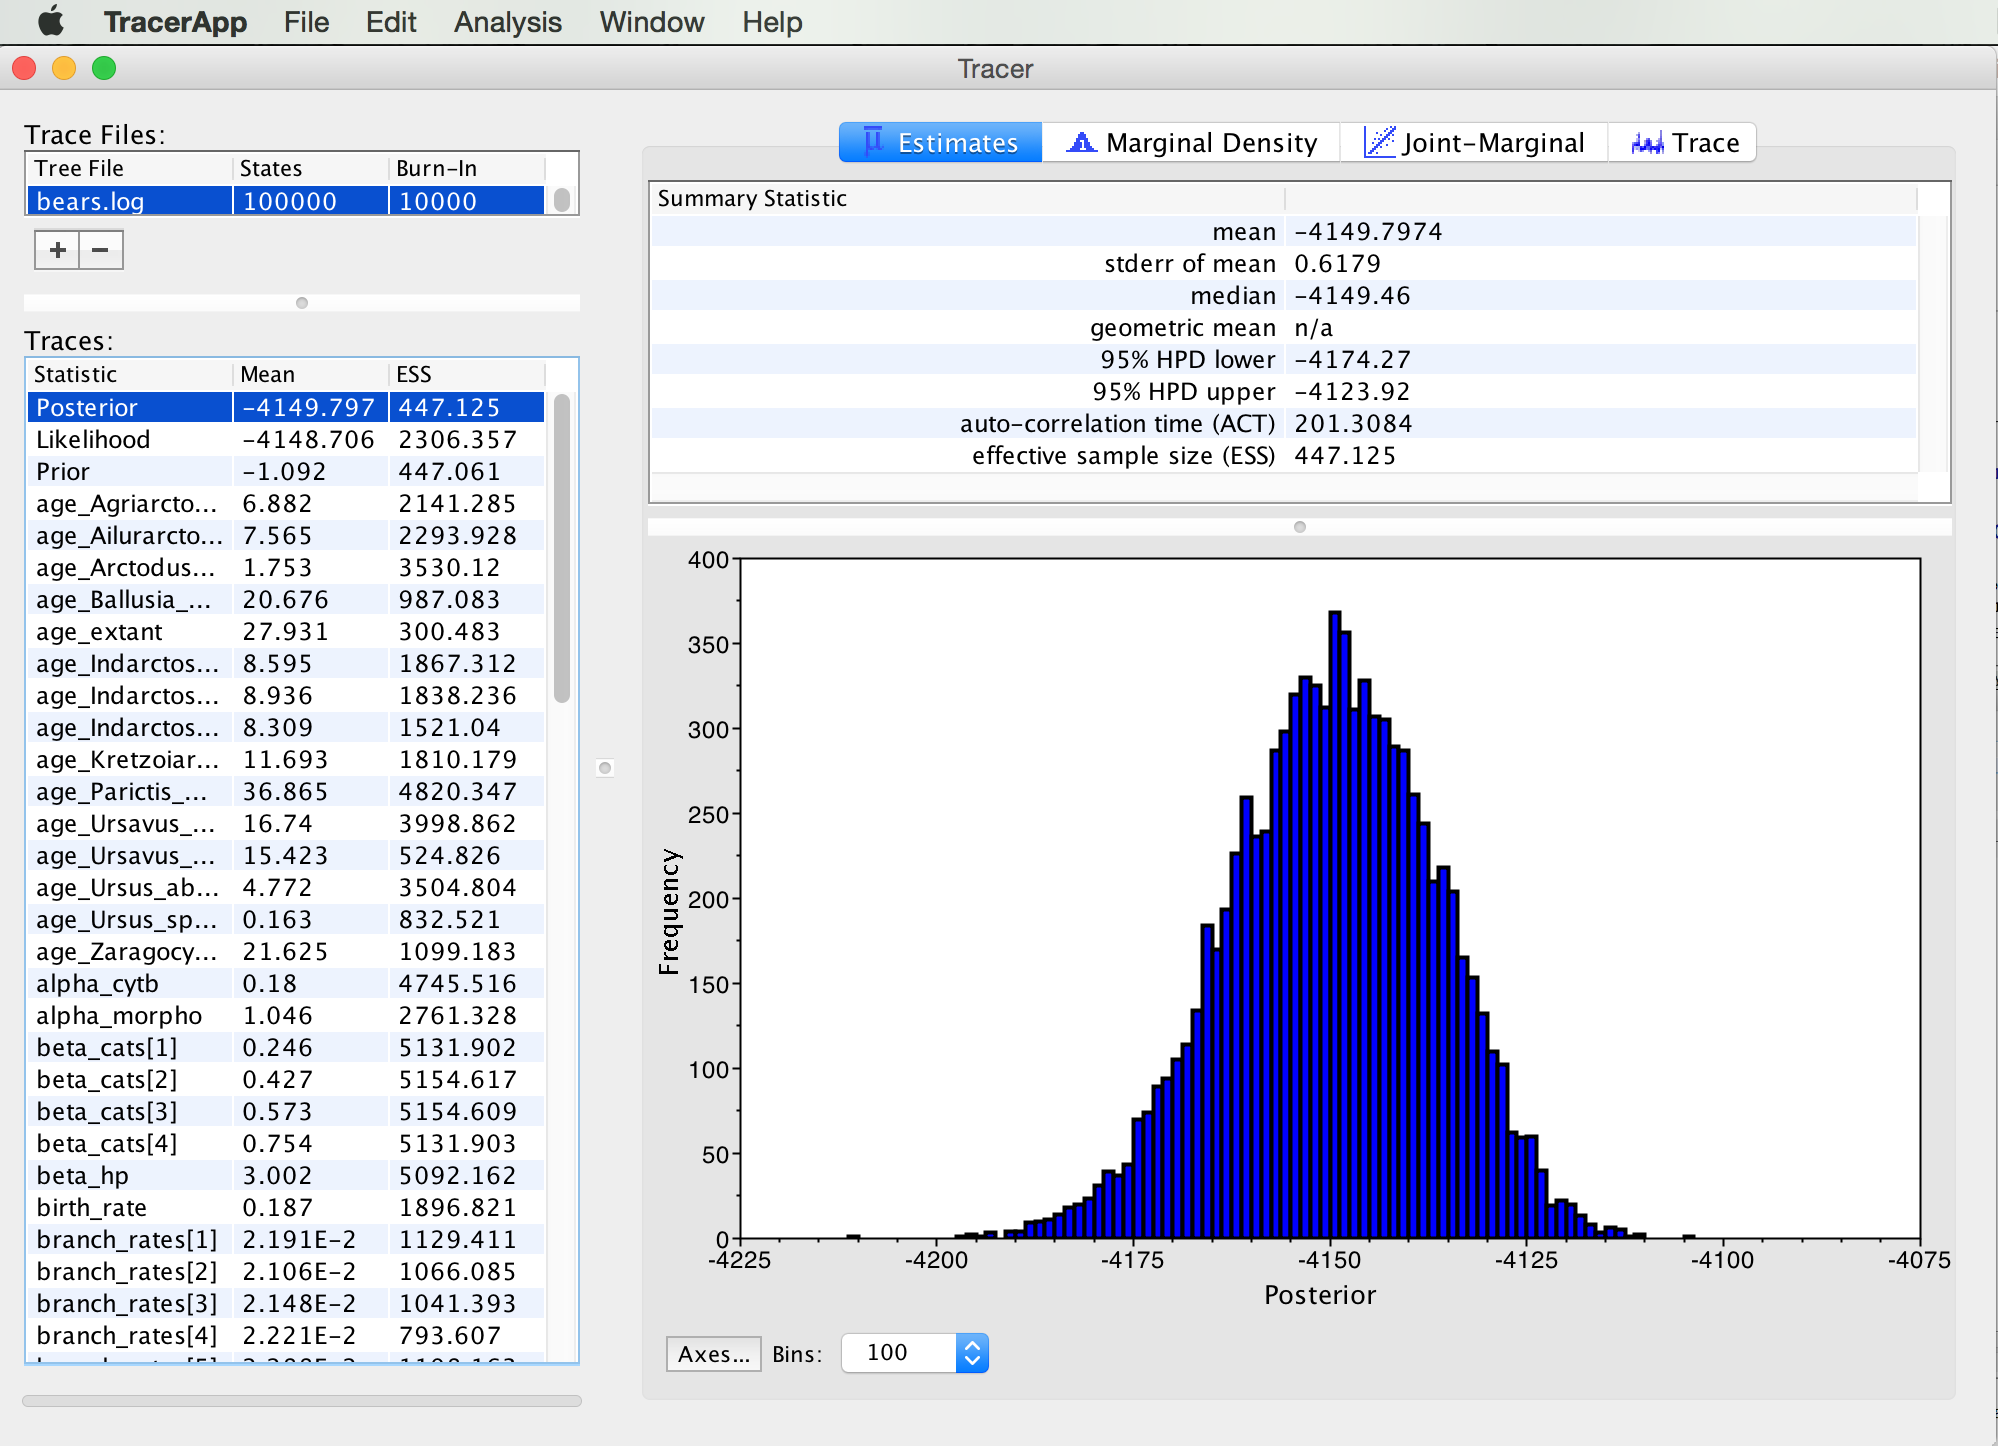
\includegraphics[width=\textwidth,angle=0]{\ResourcePath figures/samplewindow}}
\caption{\small The Estimates window. The left-hand window provides mean and ESS of the chain. The right-hand window visualizes the distribution of samples.}
\label{fig:tracer}
\end{figure}
Take a look at some of the parameters.
Are there any that have really low ESS? Why do you think that might be?

Next, we can click over to the Trace window.
This window shows us the estimates for a given parameter, ordered by position in the chain.
The left side of the chain often has a portion of the chain shaded out. This is referred to as ``burn-in''.
The idea of burn-in is that an MCMC may not immediately begin sampling from the true distribution of values, particularly if the starting condition of the chain is poor.
Therefore, these values are often discarded (or `burned'). \par
\begin{figure}[h!]
\centering
\fbox{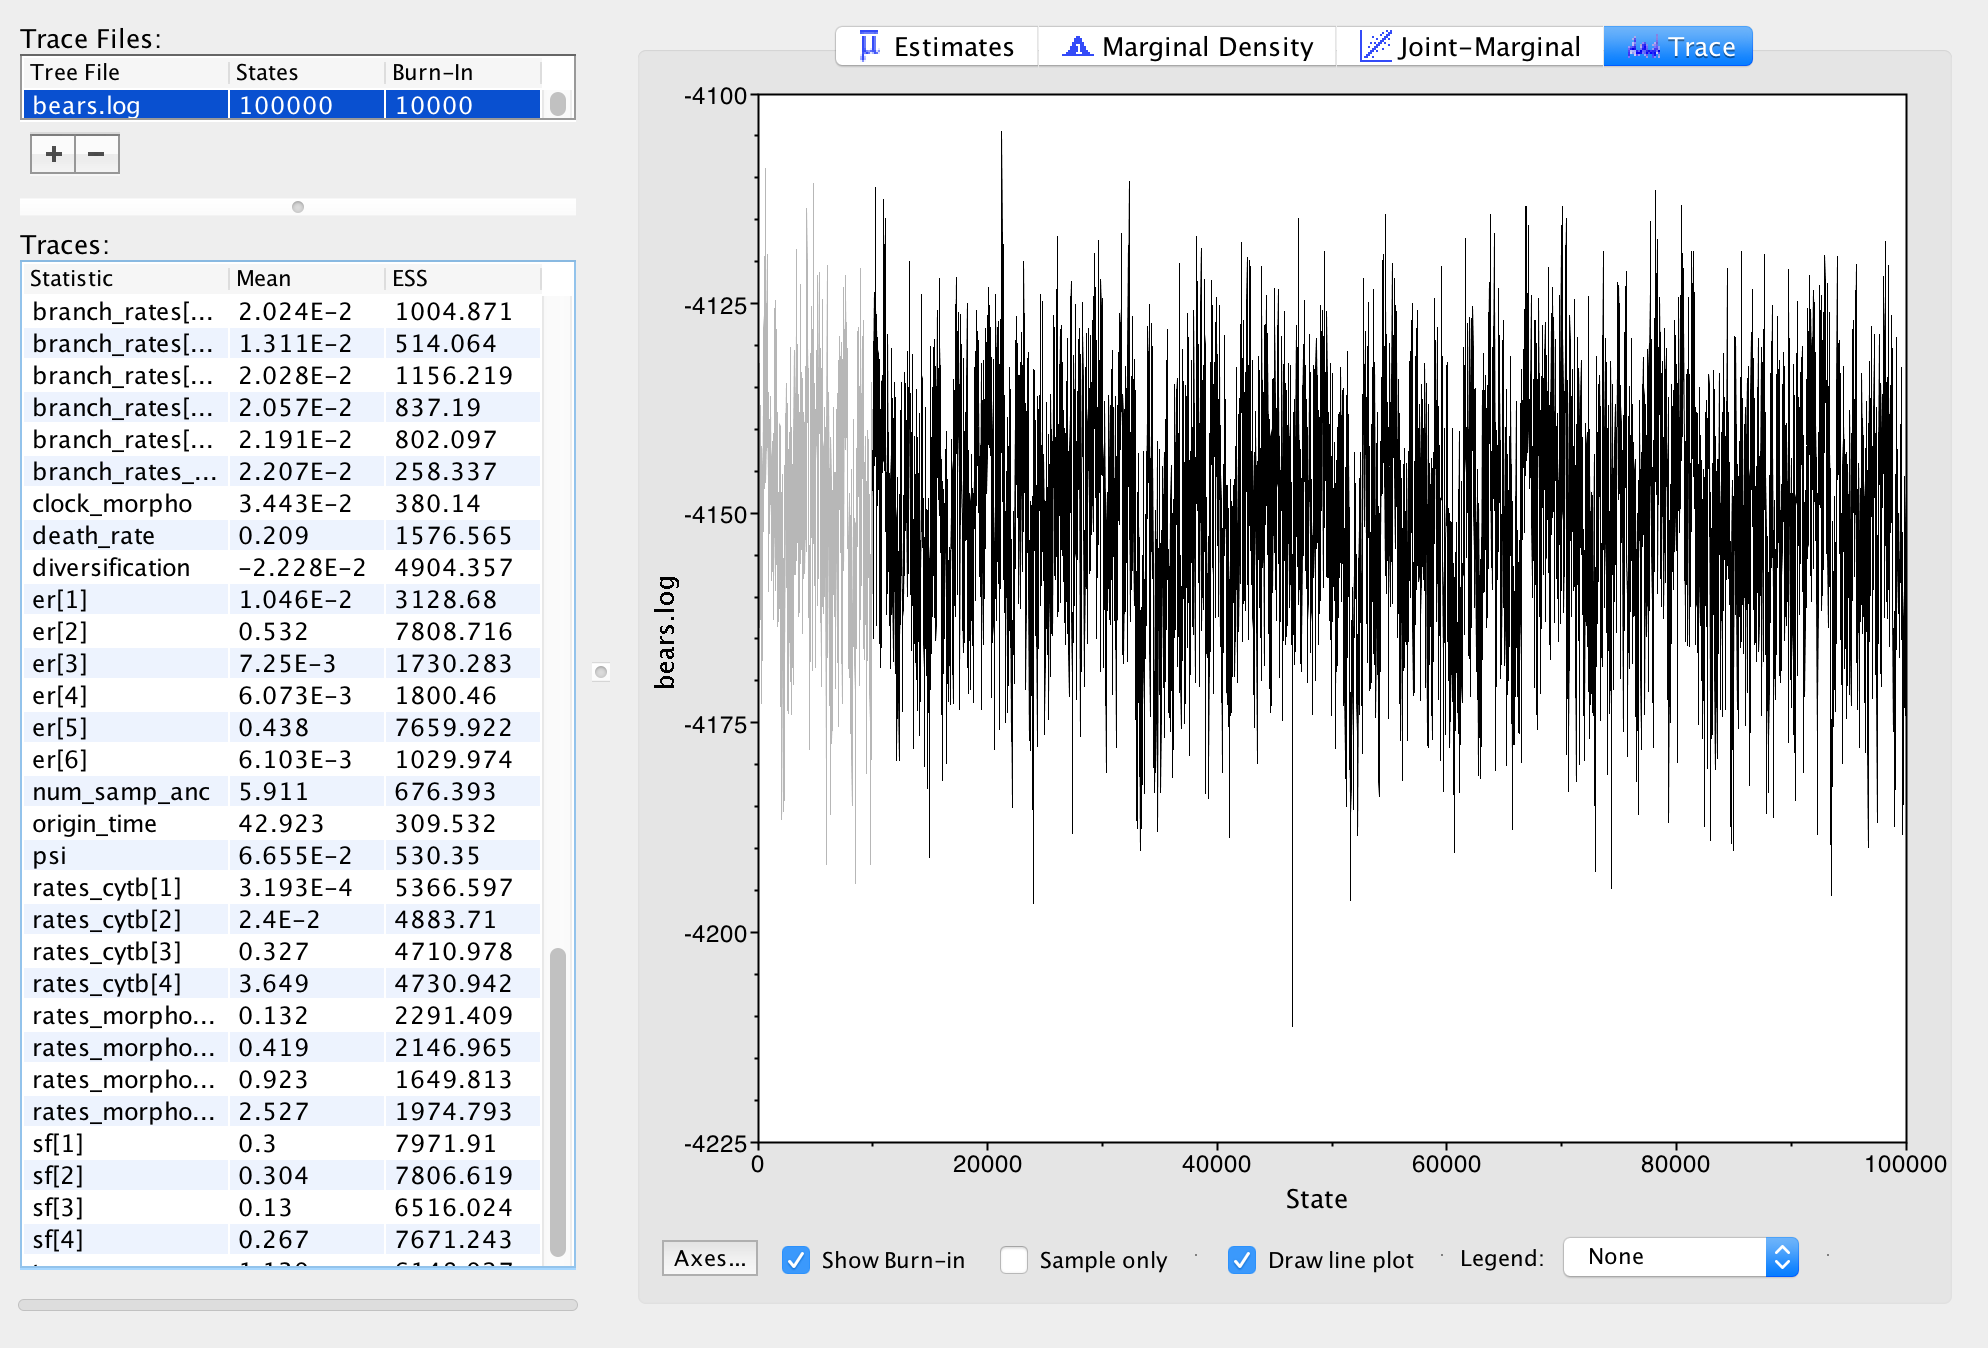
\includegraphics[width=\textwidth,angle=0]{\ResourcePath figures/trace}}
\caption{\small The trace window. The Y-axis is an estimate of the parameter being sampled (in this case likelihood score) and the X-axis is position in the MCMC chain.}
\label{fig:tracer}
\end{figure}
The trace window allows us to evaluate how well our chain is sampling parameter space.
The output in Figure 4 is a fairly good trace - there is no consistent pattern or trend in the samples, nor are the large square-shaped steps in the trace.
The presence of a trend, or of large leaps in a parameter value might indicate that your MCMC is not mixing well.
You can read more about MCMC tuning and improving mixing in the tutorial RB\_MCMC\_Intro\_Tutorial and RB\_MCMC\_Tutorial.

Are there any parameters in your log files that show trends or large leaps? What steps might you take to solve these issues?

\medskip
\subsubsection{Summarize Tree}\label{subsub:RB-SummarizeTree}

%TODO this they can do interactively in rb

Start up RevBayes at the command line.
You should do this from within the \cl{RB\_TotalEvidenceDating\_FBD\_Tutorial} directory.
We will use functions implemented in RevBayes to summarize our trees.
{\tt \begin{snugshade*}
\begin{lstlisting}
./rb
\end{lstlisting}
\end{snugshade*}}

Read in the MCMC sample of trees from file.
The first thing we need to do is remove taxa for which we did not have any molecular or morphological data.
These taxa haven't been placed on the tree due to their actual phylogenetic relationships, so it would be misleading to include them in a  summary tree.
We will use the \cl{fnPruneTree} function to remove them.
Then we will use the mccTree function to return a maximum clade credibility (MCC) tree.
The MCC tree is the tree with the maximum product of the posterior clade probabilities.
When considering trees with sampled ancestors, we refer to the maximum sampled ancestor clade credibility (MSACC) tree \citep{Gavryushkina2016}.

{\tt \begin{snugshade*}
\begin{lstlisting}
trace = readTreeTrace("output/bears.trees")

for(i in 1:trace.size())
{
    trees[i] = fnPruneTree(trace.getTree(i), pruneTaxa=v(taxa[17],taxa[20]))
}

trace_pruned = treeTrace(trees)
mccTree(trace_pruned, "output/bears.mcc.tre" )
\end{lstlisting}
\end{snugshade*}}

When there are sampled ancestors present in the tree, visualizing the tree can be fairly difficult in traditional tree viewers.
We will make use of a browser-based tree viewer called \href{http://tgvaughan.github.io/icytree/}{IcyTree}.
This tree viewer has the ability to view sampled ancestor trees, as well as many other nice abilities for tree visualization. Navigate to the page and open the tree. 

Try to replicate Fig. \ref{fig:IcyTreeSumm}. Hint: Look under style, at ``Mark Singletons''.
Why might a node with a sampled ancestor be referred to as a singleton?
Try clicking on a branch.
What are the fields telling you?
Are the ages of the fossil tips the same as what was shown in Tracer? 

\begin{figure}[h!]
\centering
\fbox{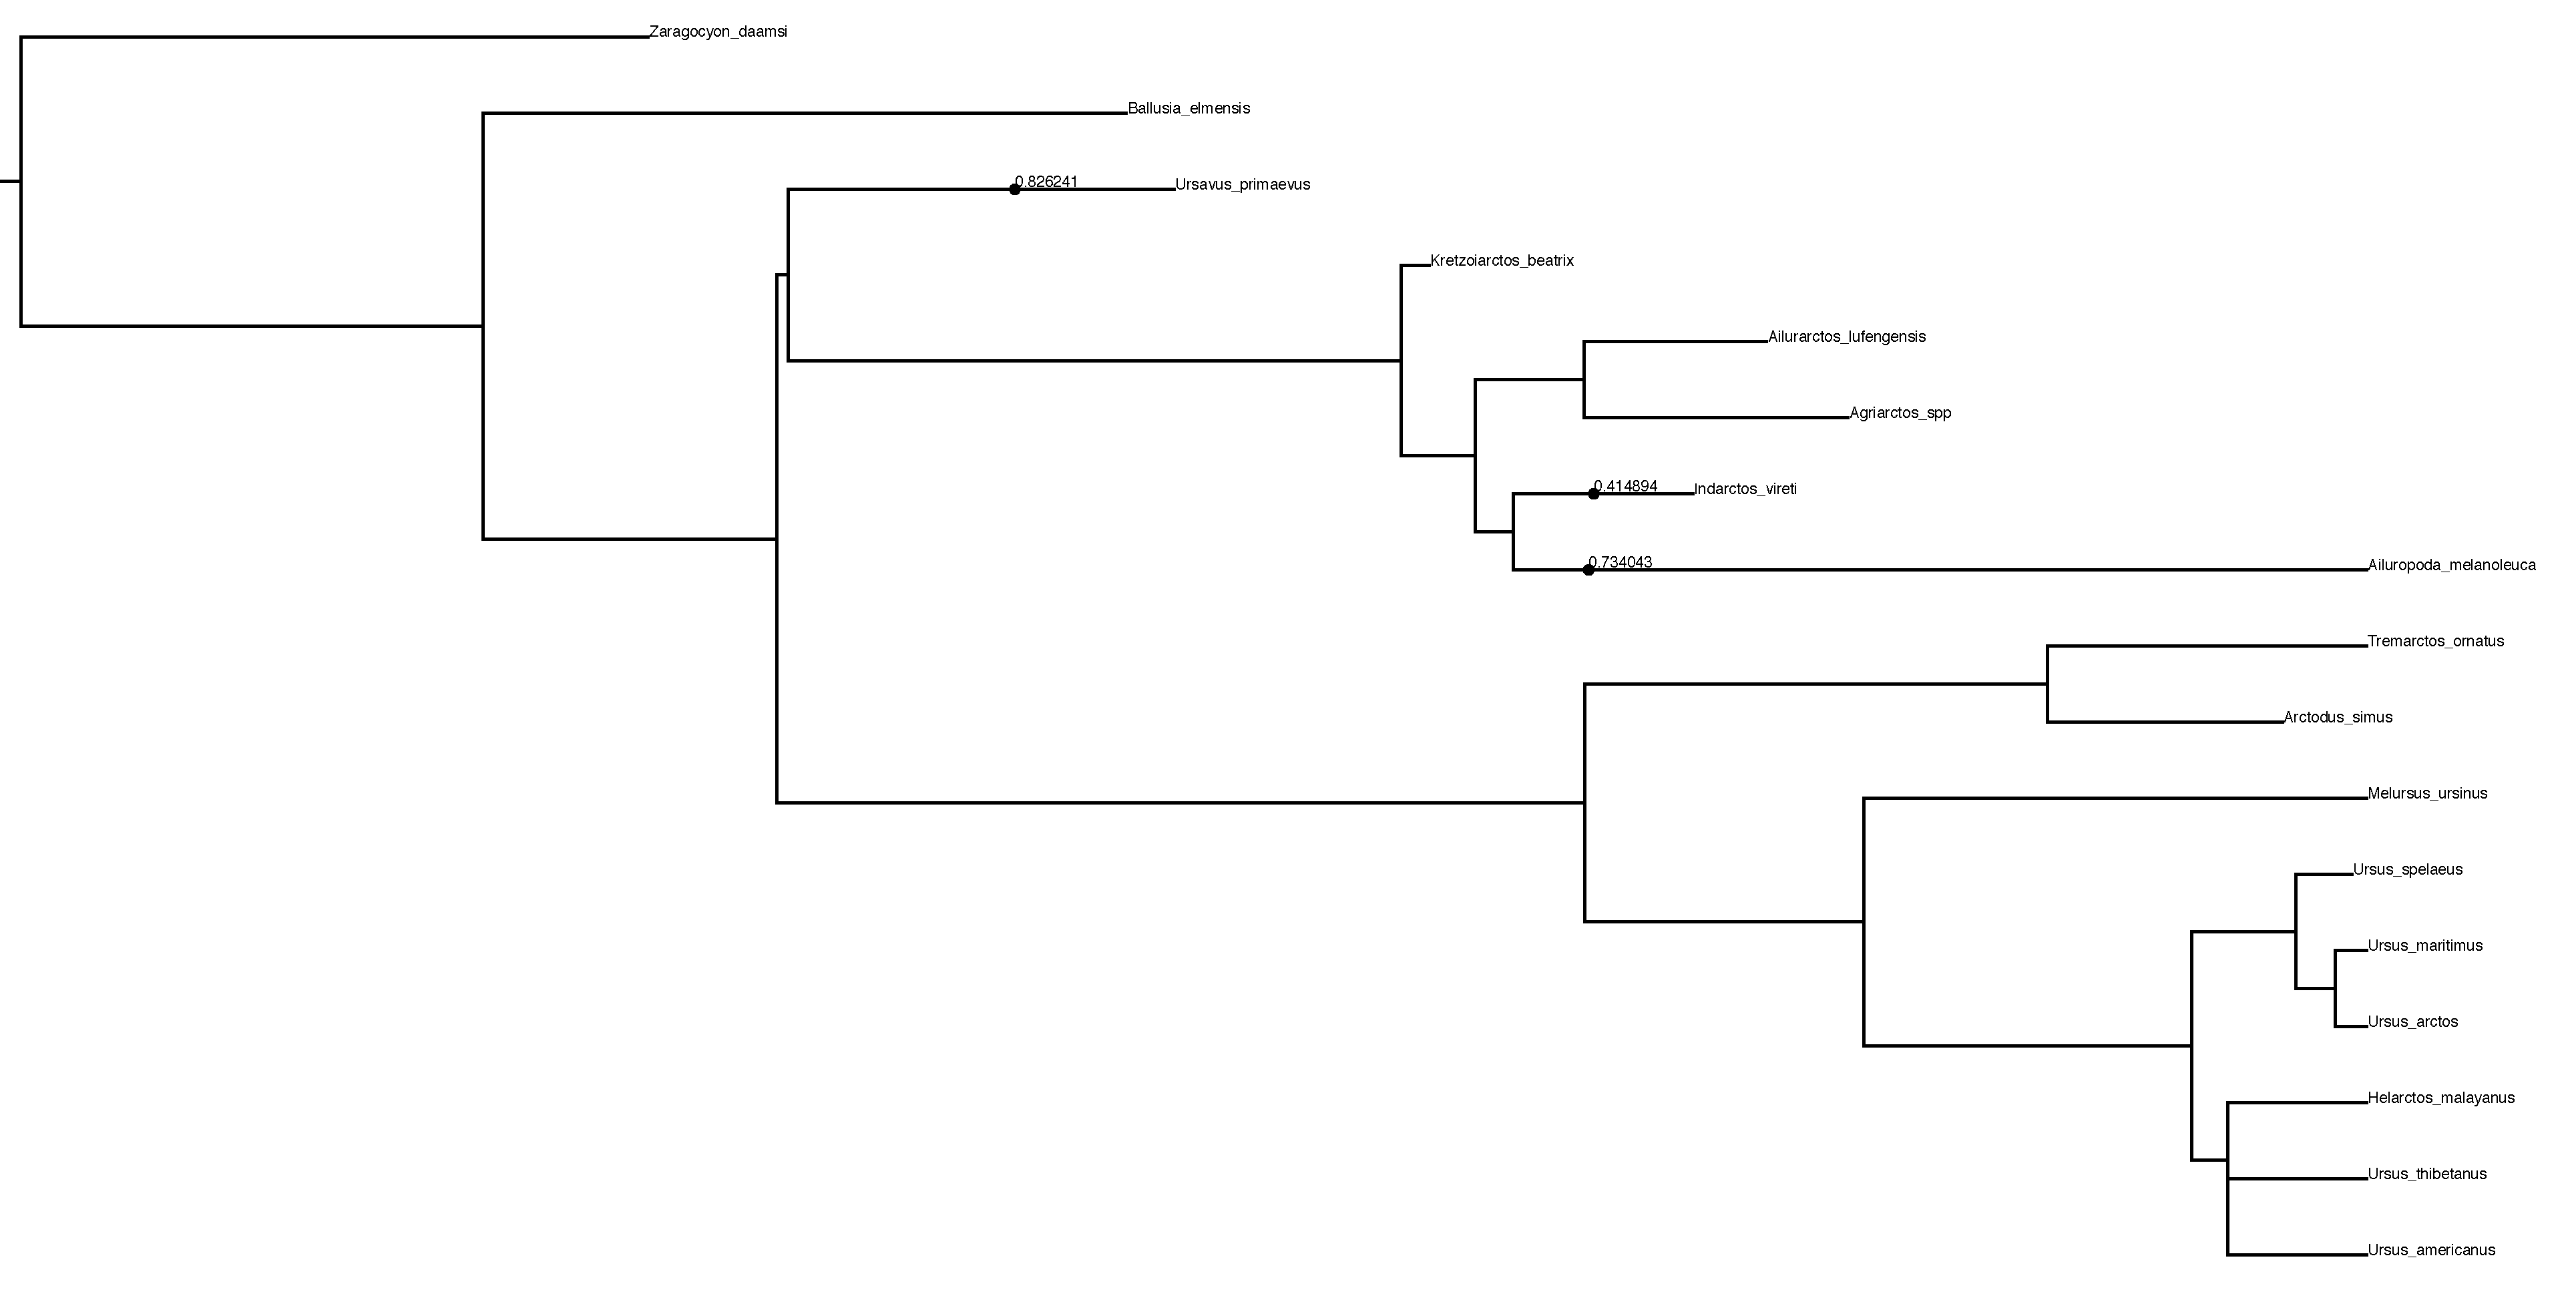
\includegraphics[width=\textwidth,angle=0]{\ResourcePath figures/summary_tree.pdf}}
\caption{\small Maximum sampled ancestor clade credibility (MSACC) tree of bear species used in this tutorial. Numbers above fossil nodes indicate the posterior probability of being a sampled ancestor.}
\label{fig:IcyTreeSumm}
\end{figure}


%TODO IcyTree

\bibliographystyle{sysbio}
\bibliography{\GlobalResourcePath refs}
